\documentclass[a4paper,12pt]{article} % тип документа

\usepackage{biblatex}
\addbibresource{sample.bib}

%  Русский язык

\usepackage[T2A]{fontenc}			% кодировка
\usepackage[utf8]{inputenc}			% кодировка исходного текста
\usepackage[english,russian]{babel}	% локализация и переносы


% Математика
\usepackage{amsmath,amsfonts,amssymb,amsthm,mathtools, textcomp} 

% Графика
\usepackage{graphicx}

% Гиперссылки
\usepackage{hyperref}
\hypersetup{
    colorlinks=true,
    linkcolor=blue,
    filecolor=magenta,      
    urlcolor=cyan,
    pdftitle={Overleaf Example},
    pdfpagemode=FullScreen,
    }
 
\usepackage{caption}
\usepackage{wasysym}

%Заговолок
\author{Петросян Акоб}
\title{ МФТИ \\ ~ \\ ~ \\ Защита информации \\ ~ \\ Безопасная подводная связь на квантовом уровне }
\date{\today}


\begin{document} % начало документа

\maketitle
\newpage

\begin{figure}
  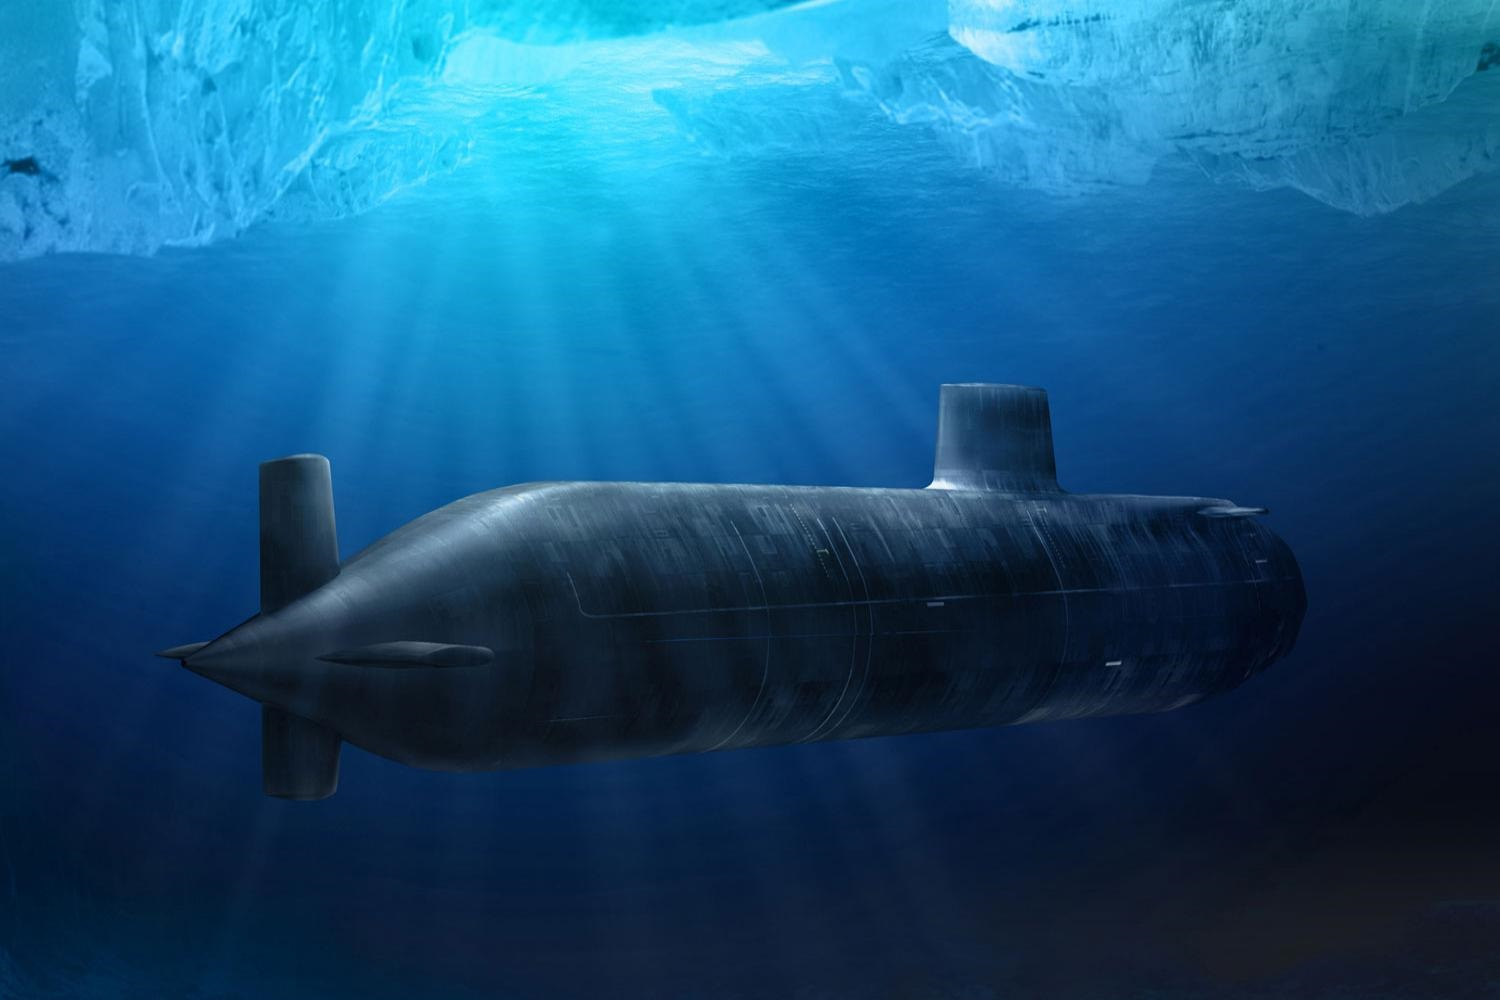
\includegraphics[width=\linewidth]{img/submarine.jpg}
  \captionof{figure}{Подводная лодка класса Astute Королевского флота является ударной подводной лодкой с ядерной установкой.}
  \label{fig:boat1}
\end{figure}

В этой обзорной статье рассмотрим некоторые из основных способов коммуникации подводных лодок. Изучим технологию квантового распределения ключей, которая позволяет подводным лодкам безопасно общаться как на глубине, так и на скорости.

\section*{Проблемы подводной связи}

\hspace{13pt} Чтобы оставаться не замеченной от гидролокаторов подводная лодка должна находиться на глубине от 60 до 100 метров. Но поддерживать подводную связь между подлодками или подлодками и базой довольно затруднительно, так как обычные радиоволны очень быстро поглощаются уже на глубине несколько десятков метров. Поэтому вместо "обычных" радиоволн используются волны с очень низкими или крайне низкими частотами(далее ОНЧ и КНЧ). Это волны, которые хорошо проникают вглубь воды, отражаются от ионосферы Земли и слабо поглощаются земной поверхностью.
~\\~

\noindent%
\begin{minipage}{\linewidth}% to keep image and caption on one page
\makebox[\linewidth]{%        to center the image
  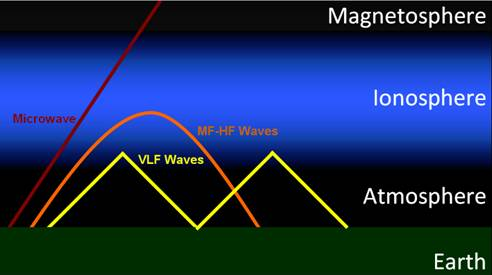
\includegraphics[keepaspectratio=true,scale=1]{img/elf_vlf.jpg}}
\captionof{figure}{ОНЧ волны}\label{SVM}%      only if needed  
\end{minipage}

~\\

Слабости такого подхода состоят в том, что чаще всего лодке надо буксировать огромные кабели-антены над водой, которых легко заметить с самолётов. Да и двигаться лодка может только с очень низкой скоростью, в определенном направлении.
~\\~

\noindent%
\begin{minipage}{\linewidth}% to keep image and caption on one page
\makebox[\linewidth]{%        to center the image
  \includegraphics[keepaspectratio=true,scale=0.35]{img/Towed_lens.png}}
\captionof{figure}{ОНЧ волны}\label{SVM}%      only if needed  
\end{minipage}

~\\

Хвастаться скоростью передачи такой метод тоже не может, так как ОНЧ и КНЧ предлагают только очень низкую полосу пропускания: ОНЧ поддерживает несколько сотен бит в секунду, а КНЧ - всего несколько бит в минуту.

Учитывая все эти недостатки, исследователи предлагают использовать технику под названием квантовое распределение ключей (КРК, {\it английский: QKD}), с помощью которой сумели добиться впечатляющих успехов не жертвуя скоростью и не заставляя подводную лодку подниматься ближе к поверхности. При этом безопасность связи гарантируется принципами квантовой механики. 

Что касается вида канала связи, ещё в 1980-х годах, были эксперименты, демонстрирующие способ поддержания оптического канала между подводной лодкой и воздушной платформой, используя оптическую связь с помощью лазера.

Группа Quantum Technologies из компании ITT Exelis, специализирующейся на оборонных технологиях, рассматривает возможность сделать еще один шаг вперед, исследуя возможность лазерной оптической связи между подводной лодкой и спутником или бортовой платформой, защищенной с помощью квантовой информации.

\section*{Квантовое распределение ключей(QKD)}

\hspace{13pt} Квантовое распределение ключей - это безопасный метод связи, реализующий криптографический протокол, включающий компоненты квантовой механики, который позволяет двум сторонам создать общий случайный секретный ключ, известный только им, который затем может использоваться для шифрования и дешифрования сообщений.

Единицей квантовой информации является кубит, который представляет собой квантовое состояние фотона. Это может быть ноль, единица или любая суперпозиция нуля и единицы.

~\\~

\noindent%
\begin{minipage}{\linewidth}% to keep image and caption on one page
\makebox[\linewidth]{%        to center the image
  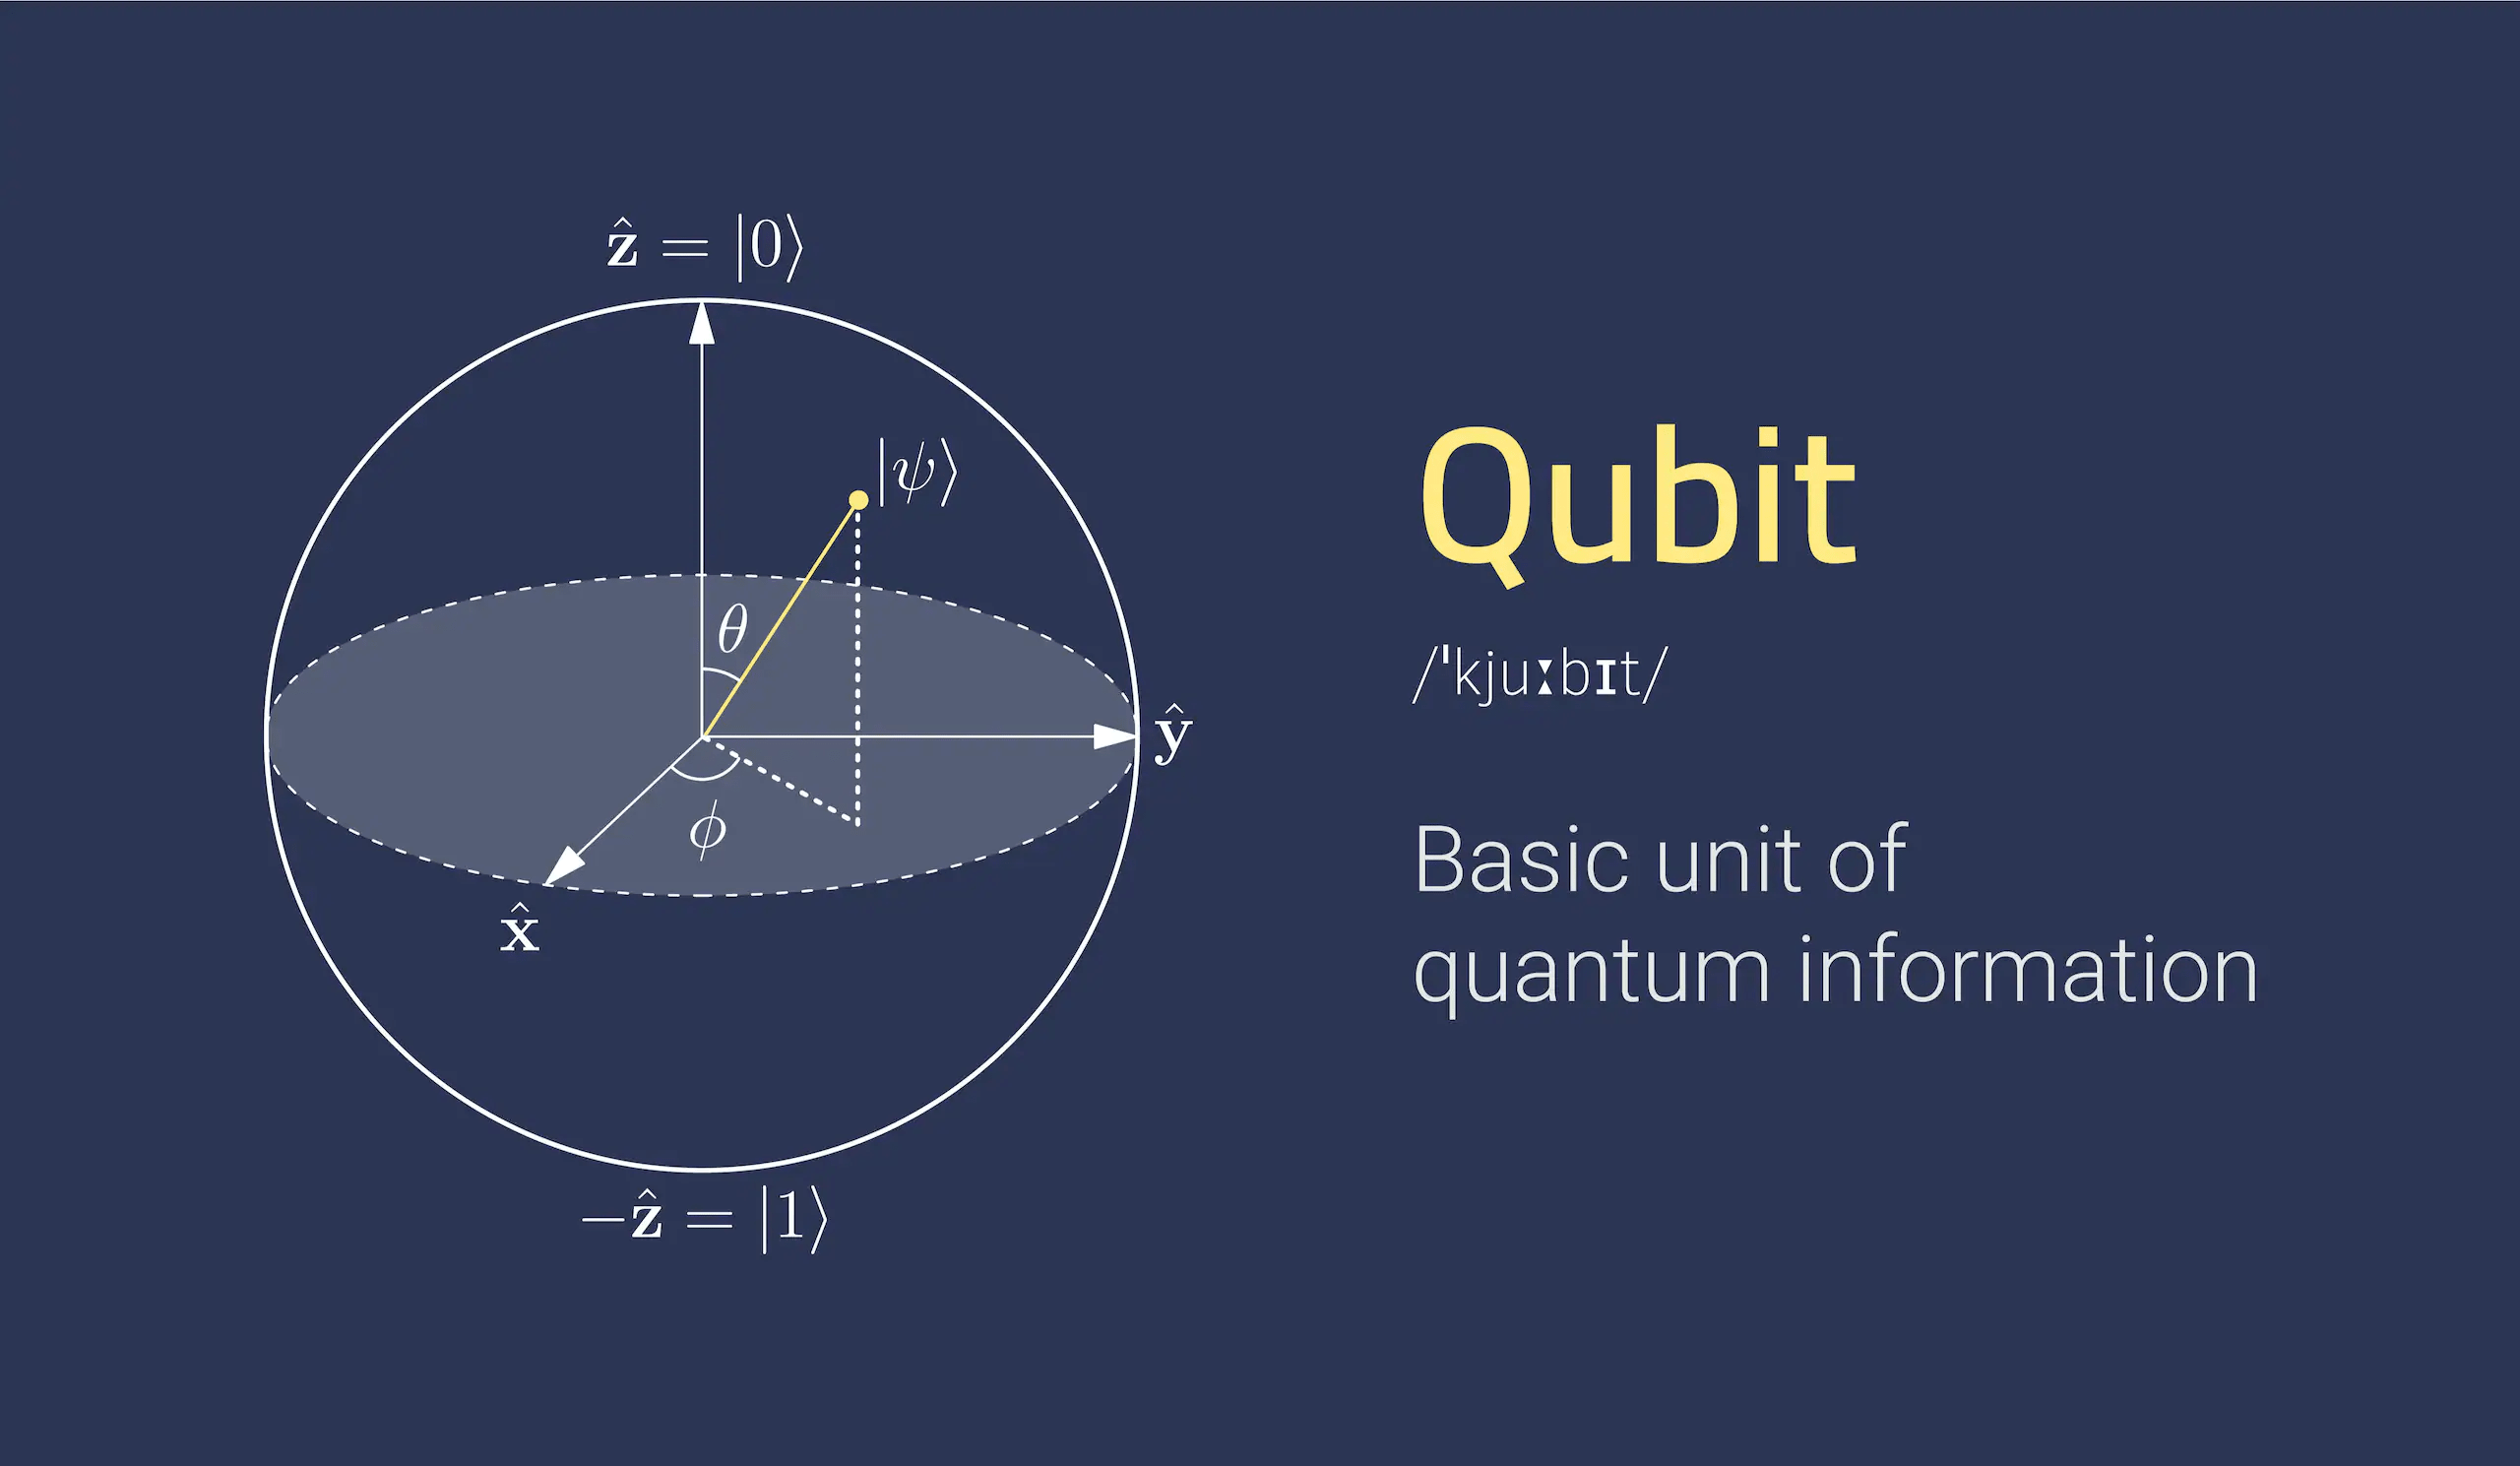
\includegraphics[keepaspectratio=true,scale=0.12]{img/qubit.png}}
\captionof{figure}{кубит}\label{SVM}%      only if needed  
\end{minipage}

~\\

Понятно, что кубит содержит в себе больше информации, чем классический бит.

Важным и уникальным свойством квантового распределения ключей является способность двух взаимодействующих пользователей обнаруживать присутствие любой третьей стороны, пытающейся получить информацию о ключе. Это является следствием фундаментального аспекта квантовой механики: процесс измерения квантовой системы в целом нарушает ее. Третья сторона, пытающаяся подслушать ключ, должна каким-то образом измерить его, тем самым создавая обнаруживаемые аномалии. Используя квантовые суперпозиции или квантовую запутанность и передавая информацию в квантовых состояниях, может быть реализована система связи, обнаруживающая подслушивание. 	

Традиционная криптография с открытым ключом , которая опирается на вычислительную сложность определенных математических функций и не может предоставить никаких математических доказательств фактической сложности обращения. В отличее от неё безопасность шифрования, использующего квантовое распределение ключей, опирается на основы квантовой механики и обладает доказанной безопасностью, основанной на теории информации, и прямой секретностью .

Главный недостаток квантового распределения ключей заключается в том, что оно обычно зависит от наличия аутентифицированного классического канала связи. В современной криптографии наличие аутентифицированного классического канала означает, что либо уже произведен обмен симметричным ключом достаточной длины, либо открытые ключи достаточного уровня безопасности. 

Квантовое распределение ключей используется только для создания и распространения ключа, а не для передачи каких-либо данных сообщения. Затем этот ключ можно использовать с любым выбранным алгоритмом шифрования для шифрования (и дешифрования) сообщения, которое затем может быть передано по стандартному каналу связи.

\section*{Заключение}

\hspace{13pt} Проведя итоги, скажу, что технология КРК имеет хорошую перспективу и в будущем, когда будут решены перечисленные выше проблемы (оптическая связь, защита от искажения состояния кубитов), можно будет добиться впечатляющих результатов, а именно невидимости подводной лодки, защищенного канала связи и высокой скорости передачи.


\section*{Литература}
\begin{enumerate}
\item Stanford VLF Group: \href{https://vlfstanford.ku.edu.tr/research_topic_inlin/introduction-vlf/}{\it What is ELF/VLF Research?}
\item Naval technology (30.01.2020): \href{https://www.naval-technology.com/features/featuredeep-secret-secure-submarine-communication-on-a-quantum-level/?utm_source=Army%20Technology&utm_medium=website&utm_campaign=Must%20Read&utm_content=Image}{\it Deep secret – secure submarine communication on a quantum level}
\item Wikipedia[electronic resource] (14.12.2021): \href{https://en.wikipedia.org/wiki/Quantum_entanglement}{\it Quantum entanglement}
\item Wikipedia[electronic resource] (14.12.2021): \href{https://ru.wikipedia.org/wiki/%D0%A1%D0%B2%D0%B5%D1%80%D1%85%D0%B4%D0%BB%D0%B8%D0%BD%D0%BD%D1%8B%D0%B5_%D0%B2%D0%BE%D0%BB%D0%BD%D1%8B}{\it Сверхдлинные волны}
\item Wikipedia[electronic resource] (14.12.2021): \href{https://en.wikipedia.org/wiki/Quantum_key_distribution}{\it Quantum key distribution}
\end{enumerate}

\end{document} % конец документа